\chapter{iOSネイティブアプリケーションのインタフェース自動生成システムの開発}
\label{chap:impl}
前述の既存UIの分析と分析から導き出したアルゴリズムをもとにiOSのネイティブアプリケーションのインタフェース自動生成システムの開発を行った.

また,普段からiOSのネイティブアプリケーションを個人開発している14-17歳の男女を被験者とした本システムの有用性をはかる実験を行い,有用性を示すことができた.

本システムの設計は以下のとおりである.
\section{システムの設計・開発}
要素,優先度,グルーピング情報からの画面のコンテンツUI自動生成システムのプロトタイプとして主要な部分のみを実装した.本研究において画面のコンテンツUIとは実際画面に表示されるUIのうち,画面遷移を司どるUI,画面のタイトル表示を除いたものを指す.

本研究のUI自動生成において重要なのは画面内の要素,優先度,グルーピング,の情報のみでUIを自動生成できることである.この点を実現するためのシステムを開発した.

本システムで利用できる要素(UIパーツ)の名称と機能は以下(表\ref{table:ui_elements})とする.名称の命名に関しては基本的にSwiftUIでの名称を使用するが,SwiftUIではテキスト表示の行数による名称の違いがないため独自に一行表示をLabel, 複数行表示をTextViewとした.
\begin{landscape}
\begin{table}[htbp]
\centering
\scalebox{1.0}{
\begin{tabular}{llllllllllllllll}
\hline
本システムでの名称                    &UIKitでの名称                    &SwiftUIでの名称                      &ユーザの操作の有無                      &主な使用用途 \\ \hline
Label &UILabel                            & Text                                     &無                                                    & 一行の文字列を表示するために使用する\\
TextView &UITextView                      & Text                                     &場合によっては有                               & 複数行の文字列を表示, 入力, 編集するのに使用する)\\
TextField &UITextField                      & TextField                              &有                                                    & 一行の文字を入力するために使用する\\
Button &UIButton                          & Button                                  &有                                                    & タップアクションを取得するために使用する \\
Toggle &UISwitch                          & Toggle                                  &有                                                    & ON/OFFの切り替えのために使用する \\
Image &UIImageVIew                   & Image                                   &無                                                    & 画像表示のために使用する\\
Map &MKMapView                    & Map                                     &有                                                    & 地図の表示のために使用する\\
DatePicker &UIDatePicker                   & DatePicker                            &有                                                    & 日付選択のために使用する\\
Slider &UISlider                           & Slider                                    &有                                                    & 特定の数値を調整するために使用する\\ \hline
\end{tabular}
}
\caption{利用可能な要素一覧}
\label{table:ui_elements}
\end{table}
\end{landscape}
\subsection{基本的な配置アルゴリズム}
前述のアルゴリズムより,基本的には要素を優先度順に縦に配置する.グループも一要素として扱い表示を行う.グループ内のレイアウトについては後述のグルーピングセクションで行う.

基本的な優先度に加え,UIの要素にはユーザからの操作を受け付けるものと受け付けないものがある.ユーザからの操作を受け付けるものに関しては指の届きやすい画面下に配置するのが適切であり,以下の表\ref{table:viewArrangementRatio}のように各要素の種類ごとに配置係数を定め,後述の優先度の値と掛け合わせた値の昇順に配置する.
\begin{table}[htbp]
\centering
\scalebox{1.0}{
\begin{tabular}{llllllllllllllll}
\hline
名称                    &配置係数 \\ \hline
Label                   &1.0\\
TextView             &0.9\\
TextField             &0.8\\
Button                 &0.5\\
Toggle                 &0.5\\
Image                  &2.0\\
Map                    &1.5\\
DatePicker          &0.7\\
Slider                  &0.7\\ \hline
\end{tabular}
}
\caption{利用可能な要素一覧}
\label{table:viewArrangementRatio}
\end{table}

\subsection{優先度}
本システムにおいて優先度からは要素の視覚的な目立たせ具合,表示順序を決定する.
優先度の値は一画面あたりの合計を10とし,それを超えた場合はスクロールする画面が提供される.
優先度による各要素の目立たせ具合は以下の通りである.以後登場するスクリーンショットは全て本システムによって自動生成されたUIである.


\subsubsection{Label}
図\ref{fig:label_priority}のように実装した.優先度5以上でもこれ以上の大きさになることはなく,余白として扱われる.

\begin{figure}[htbp]
  \begin{minipage}{\hsize}
    \begin{center}
       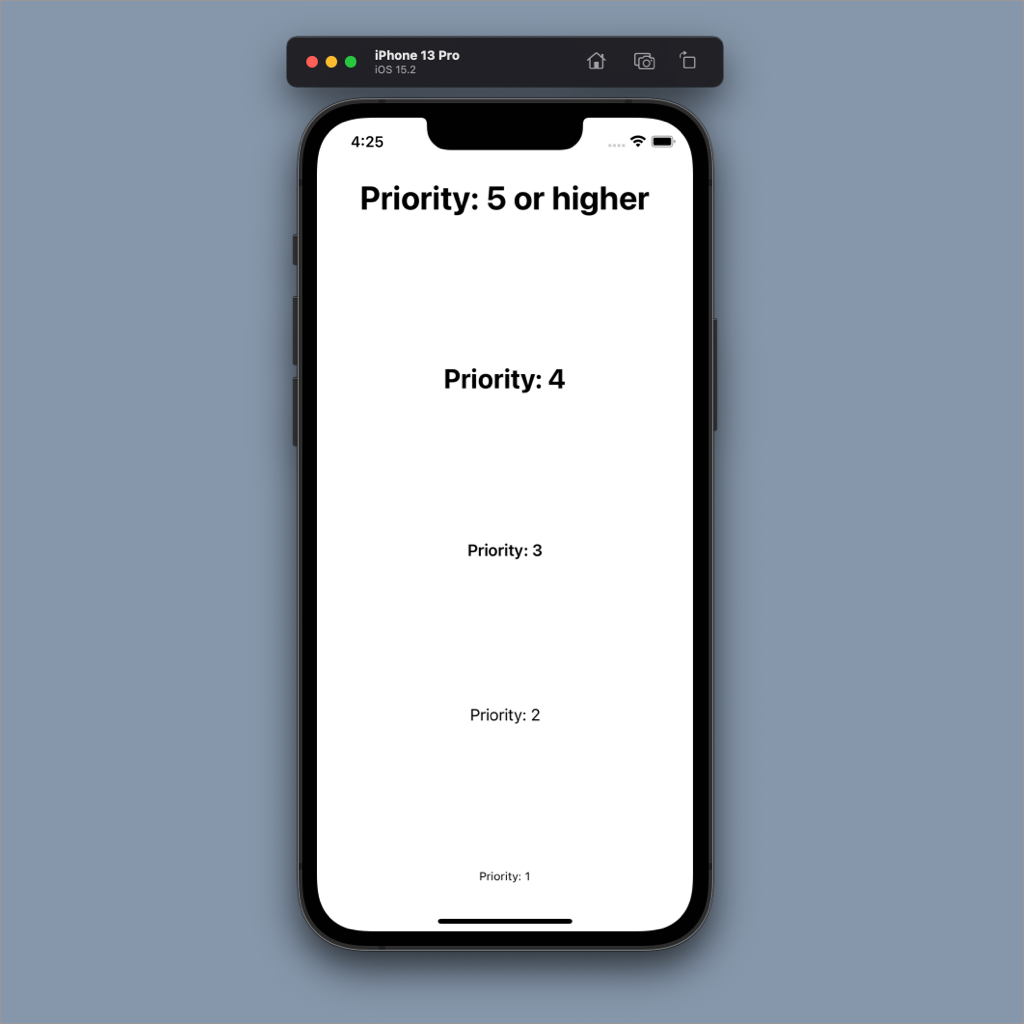
\includegraphics[width=100mm]{img/Label_priority.png}
    \end{center}
    \caption{Labelの優先度による視覚的目立たせ具合}
    \label{fig:label_priority}
  \end{minipage}
\end{figure}

\subsubsection{TextView}
図\ref{fig:TextView_priority}のように実装した.優先度5以上でもこれ以上の大きさになることはなく,余白として扱われる.

\begin{figure}[htbp]
  \begin{minipage}{\hsize}
    \begin{center}
       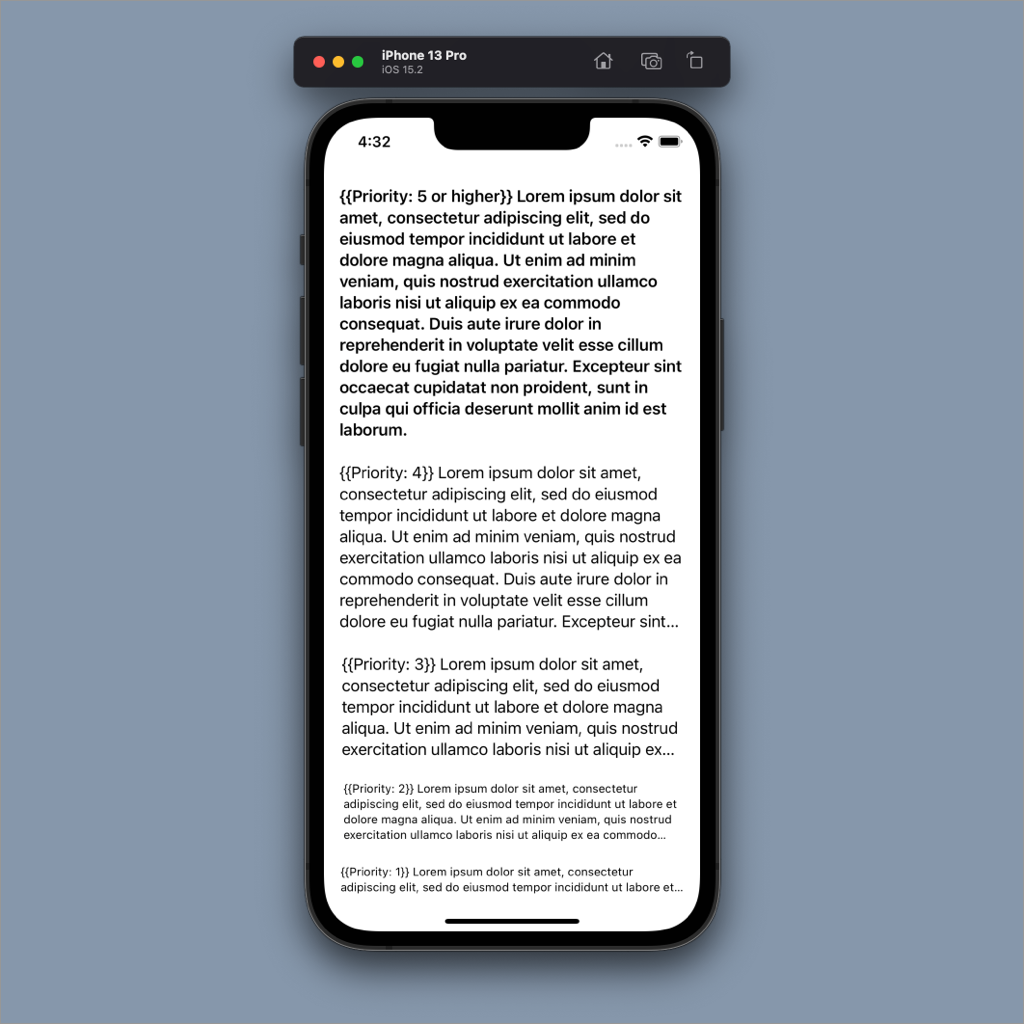
\includegraphics[width=100mm]{img/TextView_priority.png}
    \end{center}
    \caption{TextViewの優先度による視覚的目立たせ具合}
    \label{fig:TextView_priority}
  \end{minipage}
\end{figure}

\subsubsection{Button}
図\ref{fig:button_priority}のように実装した.優先度5以上でもこれ以上の大きさになることはなく,余白として扱われる.

\begin{figure}[htbp]
  \begin{minipage}{\hsize}
    \begin{center}
       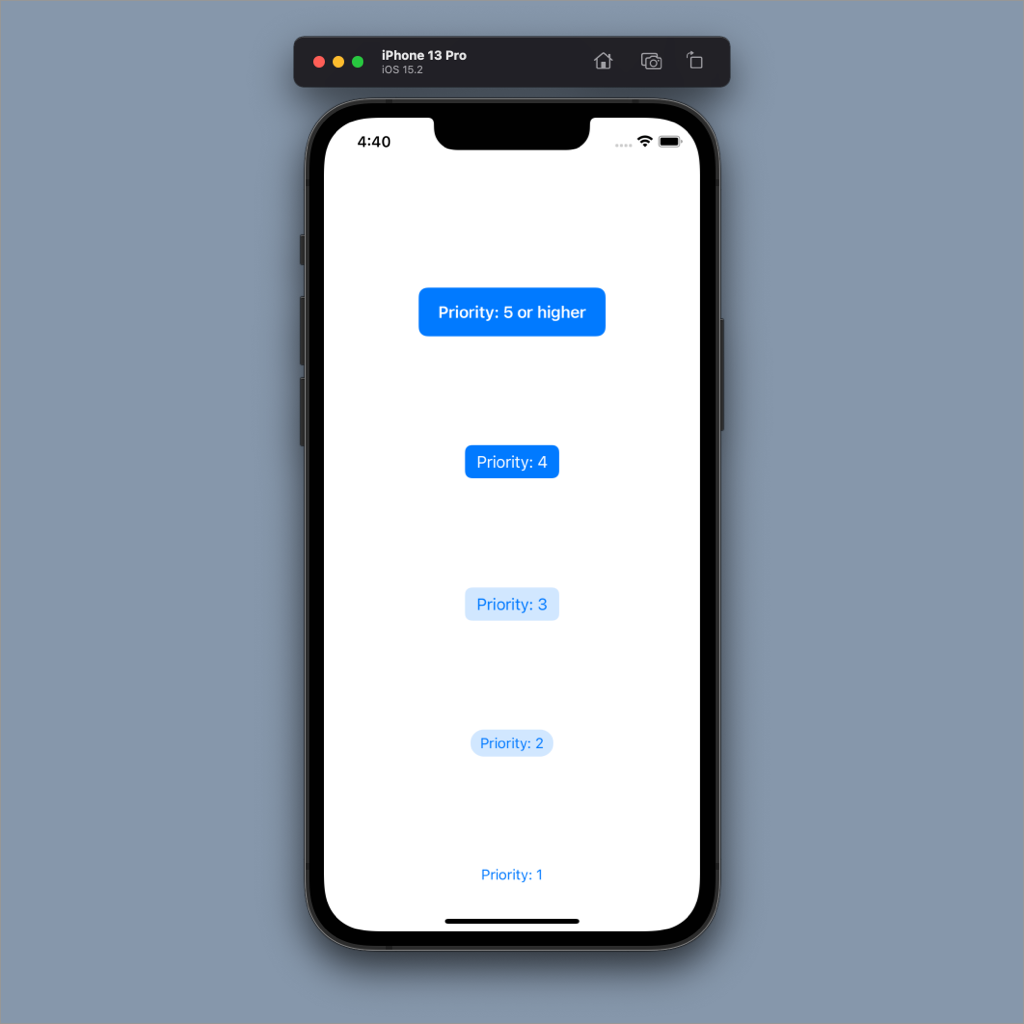
\includegraphics[width=100mm]{img/Button_priority.png}
    \end{center}
    \caption{Buttonの優先度による視覚的目立たせ具合}
    \label{fig:button_priority}
  \end{minipage}
\end{figure}

\subsubsection{Toggle}
図\ref{fig:button_priority}のように実装した.優先度5以上でもこれ以上の大きさになることはなく,余白として扱われる.

\begin{figure}[htbp]
  \begin{minipage}{\hsize}
    \begin{center}
       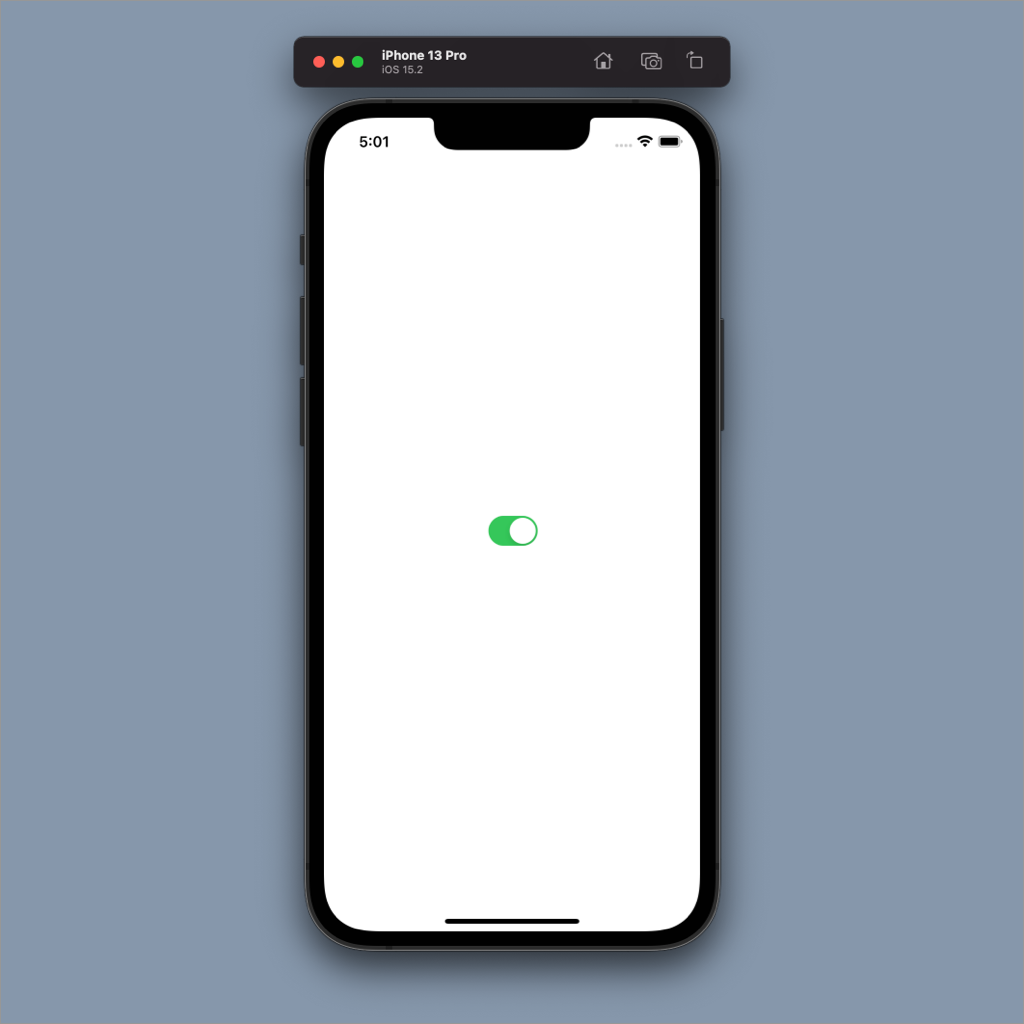
\includegraphics[width=100mm]{img/Toggle_priority.png}
    \end{center}
    \caption{Toggleの優先度による視覚的目立たせ具合}
    \label{fig:toggle_priority}
  \end{minipage}
\end{figure}

\subsubsection{Image}
図\ref{fig:image_priority}のように実装した.優先度5以上でもこれ以上の大きさになることはなく,余白として扱われる.

\begin{figure}[htbp]
  \begin{minipage}{\hsize}
    \begin{center}
       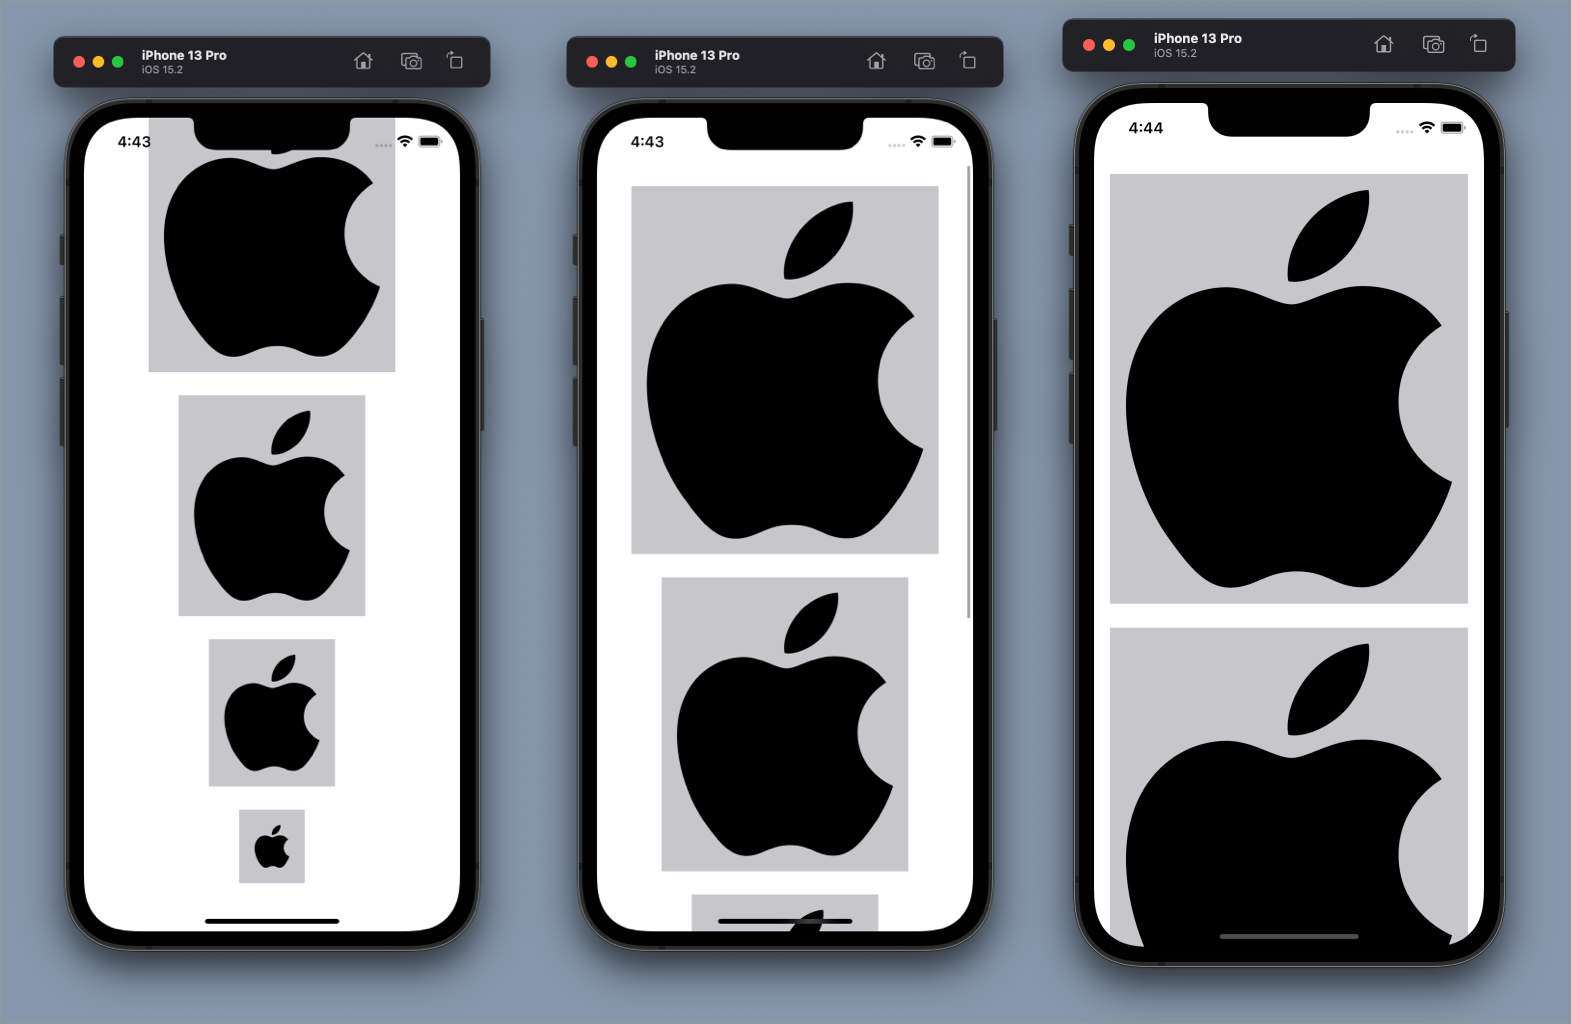
\includegraphics[width=100mm]{img/Image_priority.png}
    \end{center}
    \caption{Imageの優先度による視覚的目立たせ具合}
    \label{fig:image_priority}
  \end{minipage}
\end{figure}

\subsubsection{Map}
図\ref{fig:map_priority}のように実装した.優先度5以上でもこれ以上の大きさになることはなく,余白として扱われる.

\begin{figure}[htbp]
  \begin{minipage}{\hsize}
    \begin{center}
       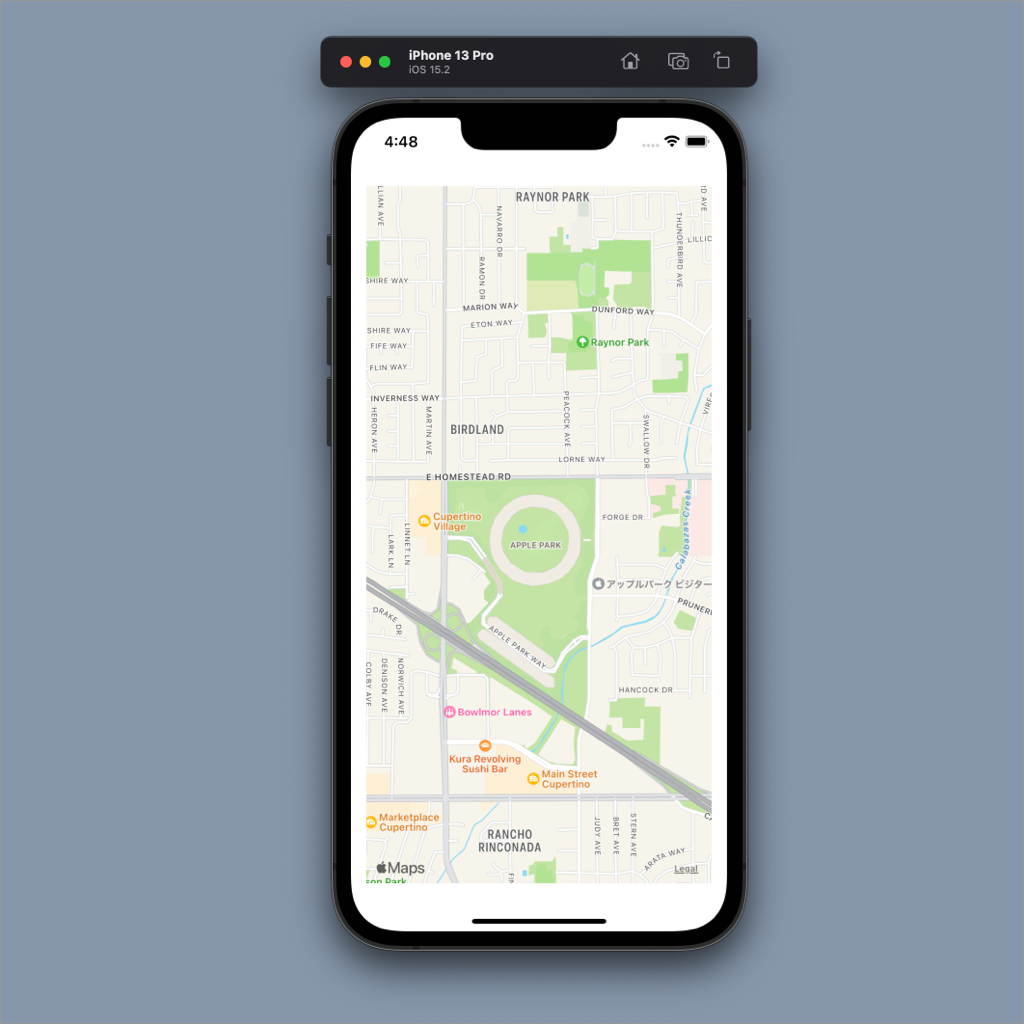
\includegraphics[width=100mm]{img/Map_priority.png}
    \end{center}
    \caption{Mapの優先度による視覚的目立たせ具合}
    \label{fig:map_priority}
  \end{minipage}
\end{figure}

\subsubsection{DatePicker}
図\ref{fig:datepicker_priority}のように実装した.優先度5以上でもこれ以上の大きさになることはなく,余白として扱われる.

\begin{figure}[htbp]
  \begin{minipage}{\hsize}
    \begin{center}
       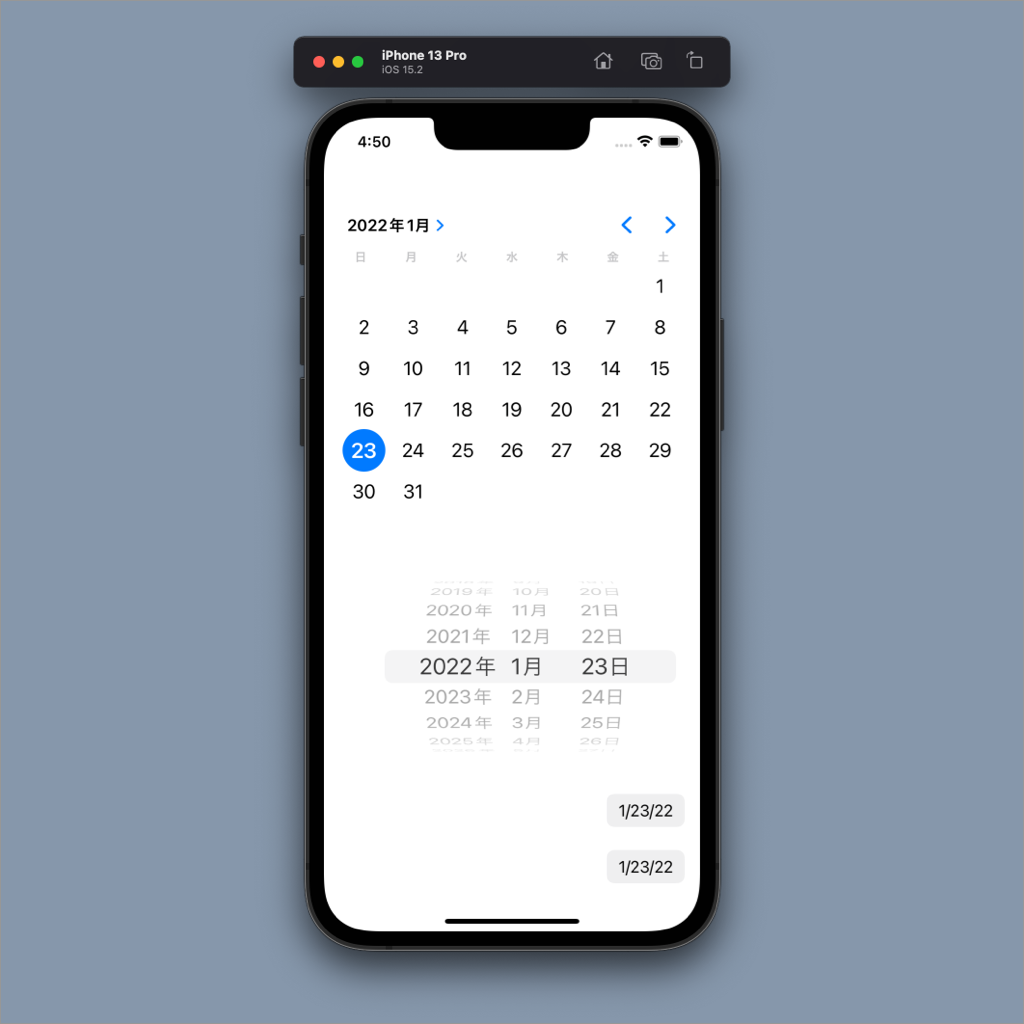
\includegraphics[width=100mm]{img/DatePicker_priority.png}
    \end{center}
    \caption{DatePickerの優先度による視覚的目立たせ具合}
    \label{fig:datepicker_priority}
  \end{minipage}
\end{figure}

\subsubsection{Slider}
図\ref{fig:slider_priority}のように実装した.優先度5以上でもこれ以上の大きさになることはなく,余白として扱われる.

\begin{figure}[htbp]
  \begin{minipage}{\hsize}
    \begin{center}
       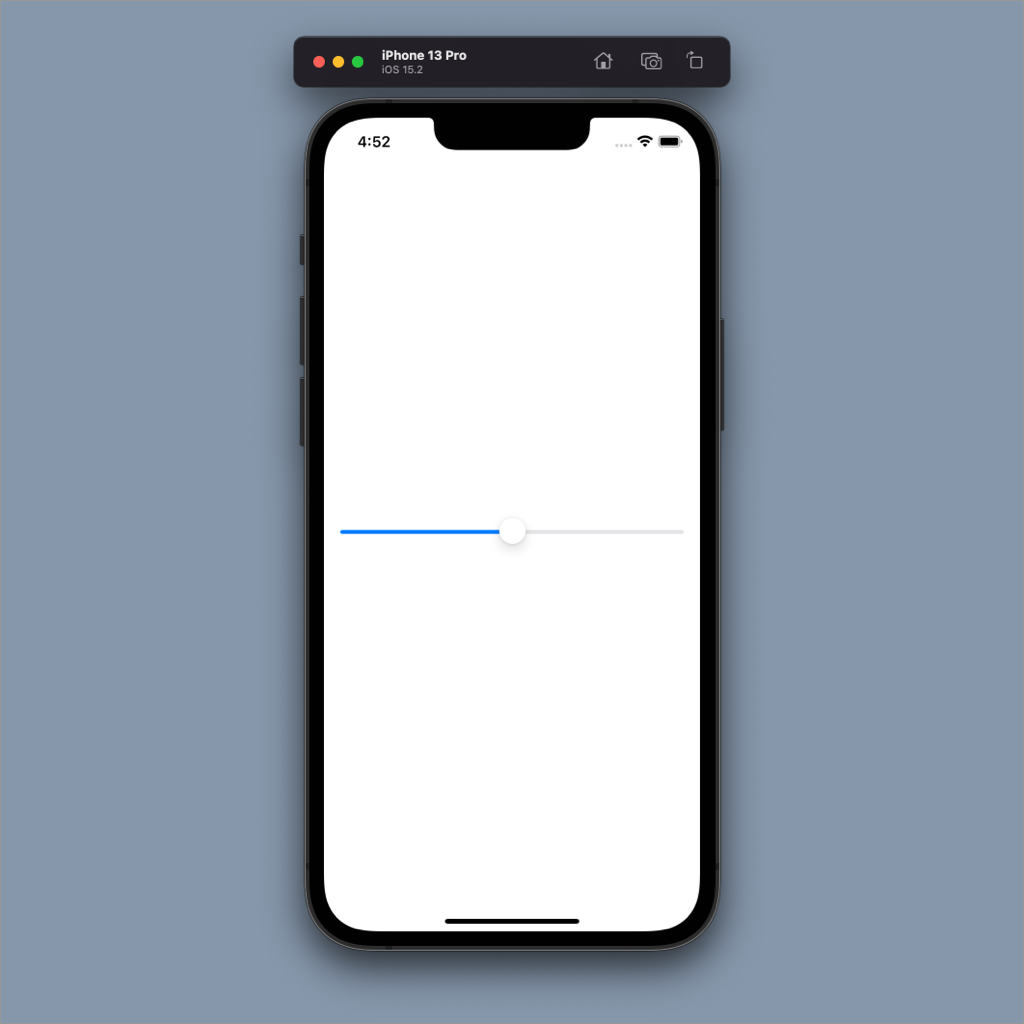
\includegraphics[width=100mm]{img/Slider_priority.png}
    \end{center}
    \caption{Sliderの優先度による視覚的目立たせ具合}
    \label{fig:slider_priority}
  \end{minipage}
\end{figure}


\subsection{グルーピング}
\subsubsection{グルーピングの入れ子構造}

\subsection{表示レイアウトアルゴリズム}

\section{既存UIの再現}

\section{システムの有効性についての実験}

\subsection{対象と手続き}

\subsection{結果と考察}